\documentclass[11pt,a4paper]{article}
\usepackage[latin1]{inputenc}
\usepackage{amsmath}
\usepackage{amsfonts}
\usepackage{mathtools}
\usepackage{array}
\usepackage{pifont}
\usepackage{ifsym}
\usepackage{booktabs}
\usepackage{listings}
\usepackage{amssymb}
\usepackage{graphicx}
\usepackage{longtable}
\usepackage{tabularx}
\usepackage{enumitem}
\usepackage{url}
\usepackage[margin=0.8in]{geometry}
\usepackage[toc,page]{appendix}
\usepackage{etoolbox}
\usepackage{morefloats}
\usepackage{multirow}
\usepackage[hidelinks]{hyperref}
\usepackage{float} % Allows putting an [H] in \begin{figure} to specify the exact location of the figure
\usepackage{verbatim}
\usepackage{listings}

\usepackage{fullpage}

\graphicspath{{img/}}

\patchcmd{\thebibliography}{\section*}{\subsection}{}{}

% Table padding
\renewcommand{\arraystretch}{1.5}

\begin{document}

\begin{titlepage}

\begin{center}

\includegraphics[width=0.5\textwidth]{img/University_Logo}\\

\textsc{\LARGE Swansea University }\\[0.5cm]
\textsc{\large MEng Computing }\\[2cm]

{ \huge \bfseries Group Project CS-M04}\\[0.2cm]
\textsc{\large Team Structure, Methodology, Requirements and Specifications}\\[1.5cm]

\begin{minipage}{0.4\textwidth}
\begin{flushleft}

\emph{Authors:}\\
Adam \textsc{Barrell} {\scriptsize \emph{(632975)}} \\
Thomas \textsc{Milner} {\scriptsize \emph{(637755)}} \\
Lewis \textsc{Hancock} {\scriptsize \emph{(xxxxxx)}} \\
Christopher \textsc{Lewis} {\scriptsize \emph{(xxxxxx)}} \\

\end{flushleft}
\end{minipage}
\begin{minipage}{0.4\textwidth}
\begin{flushright}

\emph{Supervisor:}\\
Parisa \textsc{Eslambolchilar}

\end{flushright}
\end{minipage}\\[1.3cm]

{\today}
\end{center}

\end{titlepage}

\newpage 

\tableofcontents

\newpage
\section{Introduction}
%- Purpose of Document (who it's for, outline Digital Trails briefly again).
%- Outline of Document (what we cover in the document).

\section{Technology Choices}
%- What APIs, Libraries, IDEs etc we are using, compared with other options we had. Argue our choices.

\subsection{The API}
To keep the Application and the website in sync, and allow for future developements such as aditional applications, an RESTful API (Application Programming Interface) was created.

\begin{description}
\item[API] Application Programming Interface, In general an API is a method of interaction between two software components through code. This often take the form of a Library, although a web API generally takes the form of several remote calls which are exposed to the user of the API. 

\item[REST] Representational State Transfer, is a architecture style which was used to design HTTP/1.1 (Hyper Text Transfer Protocol Version 1.1) and the URI (Universal Resource Identifier) standards. It consists of a set of constraints on components, data and there connections. The primary constraint is a Client-Sever separation, with the server being responsible for data storage, and the client responsible for the user interface and user state. The server is also required to be stateless which means no client context can be stored on the server.
\end{description}

For the API the Slim Framework\cite{slim} was chosen. This framework is designed for creating lightweight restful API's and websites and provides a versatile and well tested bases for the work. There were several other choises for this framework, but Slim was chosen becouse it was the most popular and well documented option. The Paris ORM(Object Relation Mapper) Framework\cite{paris} was also chosen to assist in database access. The ORM uses simple database models to reduce the steps in the process of interacting with the database. This framework makes it very easy to work with databases, drastically cutting the code needed to retrieve data and process it into objects. For example, if you had a simple database with just Documents and Users it would be possible to model this using just the code below. There are two model definitions and then 2 very basic lines of code which return a user object in the variable \lstinline{$user}. The second line then queries \lstinline{$user} to get all the documents associated with that user. \cite{TomMilestone2} 

\begin{lstlisting}
class User extends Model {
	public function documents(){
		return $this->has_many('Document');
	}
}

class Document extends Model{
	public function user(){
		return $this->belongs_to('User');
	}
}

$user = Model::factory('User')->find_one($id); 
$documents = $user->documents()->find_many();
\end{lstlisting}

\subsection{The Server}
The project is currently hosted on an Amazon EC2 server owned by a group member. Having a private server like this has allowed us to configure it as we require. The server is currently running Ubuntu Linux with Apache webserver, PHP and MySQL database installed. Git is used to push documents up to the server which are then automatically coppied into the correct folder for the webserver. Each part of the project can then be given a unique subdomain for testing purposes. Currently the API is hosted at \url{http://whiterockapi.tmilner.co.uk/} and the Web Portal is at \url{http://whiterock.tmilner.co.uk}.


\section{Project Progress}
%- THIS IS THE OVERVIEW SECTION
%- Show the subsystem designs and explain the current structure of the project. 
%- Possible to move the risk management and schedule sections up here if people feel it reads better. Depends how big those sections get.
%- Mention Amazon EC2 for testing purposes

\subsection{Database}

%- Why do we need a database, what data will it store?
A relational database has been created to store persistent data for the web portal and Android application.
The database stores data relating to entities such as walks, way points, users and media locations.
The database is currently hosted by an Amazon EC2 server (see technology choices) using MySQL.

%- How was the database designed?
The database schema was designed using Visual Studio's entity designer which allows developers visually develop databases.
This tool allows tables to be created on a canvas where relationships and attributes can be modified.
A table was created for each entity or concept that required persistent storage as shown in Figure \ref{fig:DatabaseSchema}.
Columns were then added to each table to represent the attributes of each entity.
For example, the \emph{EnglishWalkDescription} table has an \emph{Id}, \emph{Title}, \emph{ShortDescription} and \emph{LongDescription}. The column \emph{Id} is mandatory for standalone entities as the rest of their properties are identified by this unique key. 

%- How was the database be generated from this model?
The Visual Studio entity designer was able to generate an SQL script to create the database from the design shown in Figure \ref{fig:DatabaseSchema}. This script was executed on the MySQL server which in turn created the tables designed in the entity designer.

%- How will the database be exposed if not directly?
The White Rock Trails database is not publicly exposed and can only be interfaced through a public facing API (see section XXXXX). 
This will ensure the robustness of the database as additional business logic from the API protects the underlying database from erroneous data and unauthorized access.

%- What applications will consume data from this database?
The web portal and Android application will both consume data from this database through the public API. 
The web portal will consume data with every request made by users from their web browser. 
In contrast, the Android application will synchronise a local copy of the database through the API. 
This ensures that the application can be used offline as many walks will not be in range of an internet access point.

%- How does it's design conform to the requirements?
The database design conforms to the requirements required by the client which are defined in the Initial Document. 
More specifically, the design shown in Figure \ref{fig:DatabaseSchema} is based on the initial schema design provided by the client. 
The initial schema contained tables that did not have a high normal form. 
English and Welsh translations were present in the same tables for both the walk and way point descriptions. 
These tables were normalised as shown in Figure \ref{fig:DatabaseSchema} by moving the English and Welsh descriptions into separate tables.
In addition, the media locations for each way point were also present in the same table.
This was normalised by moving different media types such as images, audio and video into tables \emph{WaypointImage}, \emph{WaypointAudio} and \emph{WaypointVideo} respectively.

%- Describe the relationships (one-one) (one-many) (many-many)
Relationships were defined between tables using Visual Studio's entity designer. 
The designer supports a range of associativities such as one-one (1-1), one-many (1-*) and many-many (*-*). 
Some of these associativities were used in the White Rock Trails schema as shown in Figure \ref{fig:DatabaseSchema}.
For example, the \emph{Walk} entity can have many \emph{WalkReviews}, one \emph{User} who created it, many \emph{Waypoints}, one \emph{EnglishWalkDescription} and one \emph{WelshWalkDescription}.

\begin{figure}[h!]
\centering
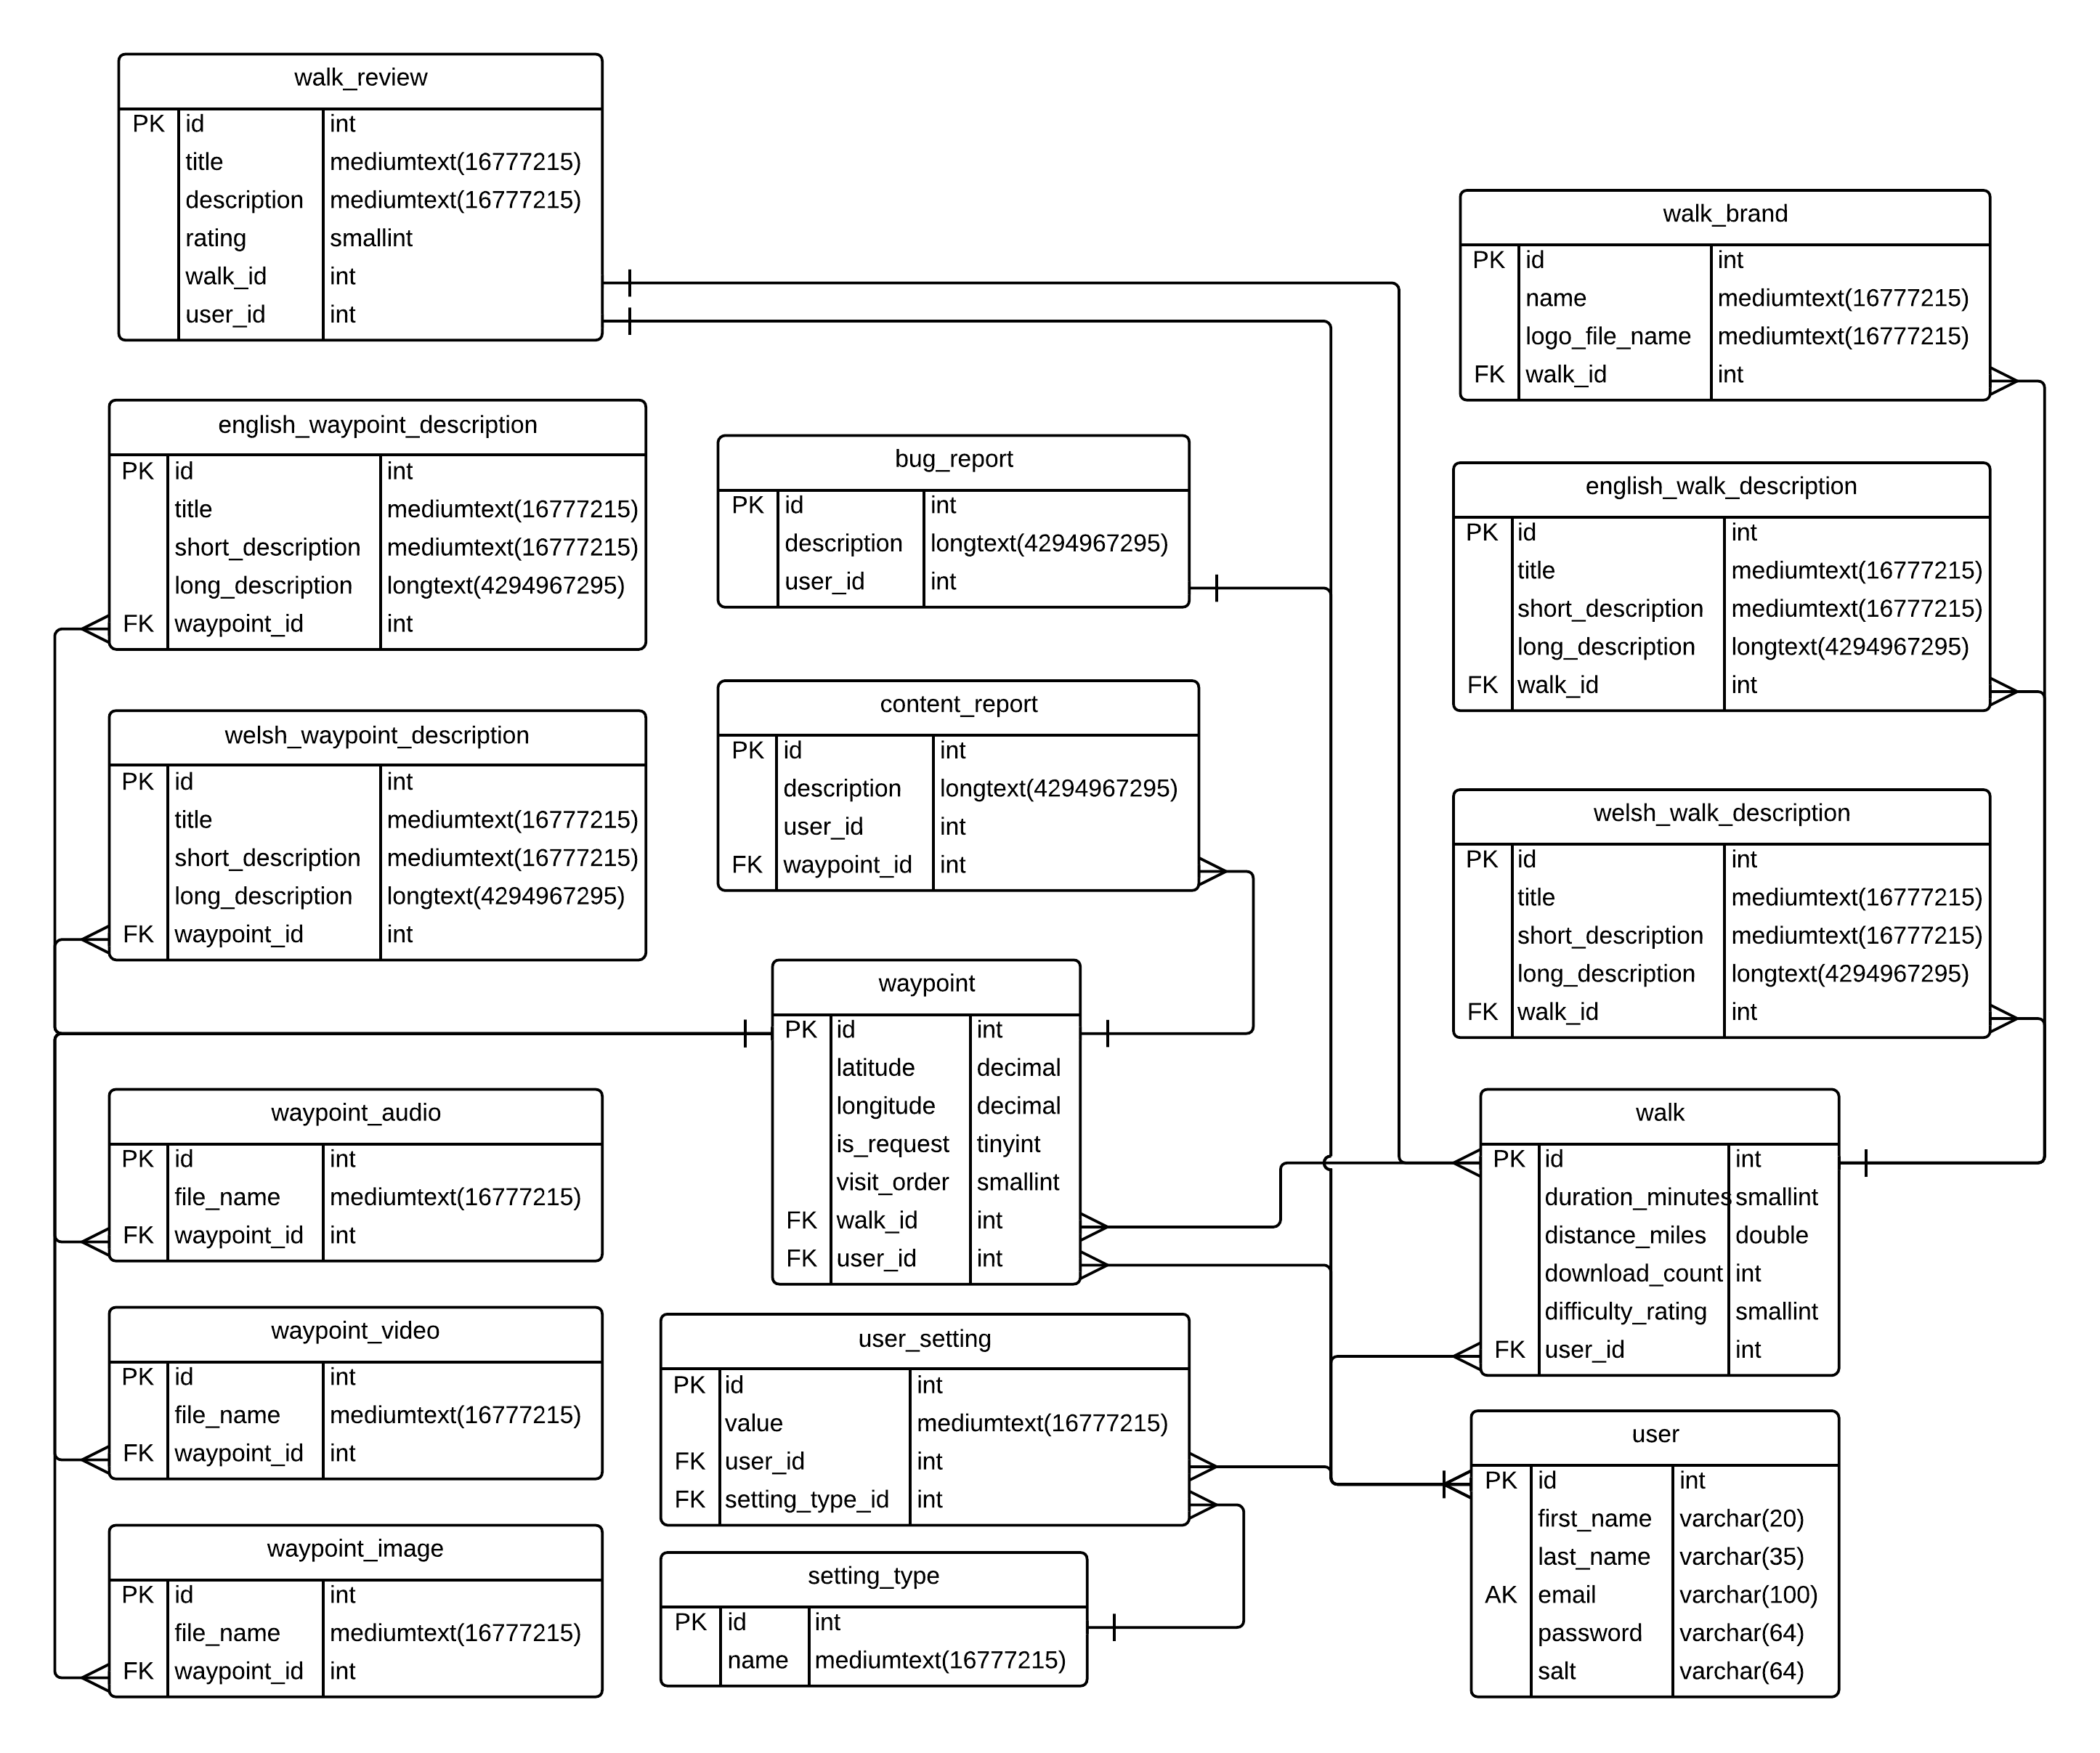
\includegraphics[angle=90, width=1\linewidth]{./img/DatabaseSchema}
\caption{Schema of the White Rock Trails relational database.}
\label{fig:DatabaseSchema}
\end{figure}


\subsection{User Interfaces}
%- Heuristic Evaluations on similar products
%-- Explain how we are doing the evaluation blahblah nielsen etc.
%-- List of tasks for evaluators to complete (we should really ALL be involved in doing the evaluations).
%-- Problems found when completing each task
%- Our prototype UI 1
%-- show how it meets reqs, how heuristics helped design.
%-- Heuristics on this etc.
%- Our prototype UI 2
%-- show it meets reqs, how heuristics helped design.
%-- Heuristics
%- repeat as necessary.

\subsection{Android Application}
%- ContentProvider
%- Authorisation
%- Google Maps
%- Current design to sync with server
%- Chris can chuck in his Fragments here, so he has some code to show.


\subsection{API}

There are several important parts to the API, first it must have a coherent set of routes/urls for acces to all if its functionality, secondly it must provide a method of authenticating users and finaly it must adhear to to principles of REST as closely as possible. 

\subsubsection{Routes}

The API is called through a series of routes, it was important to make these routes as simple and coherant as possible.

\begin{longtable}{p{0.45\textwidth}|p{0.35\textwidth}|p{0.1\textwidth}}\hline
    \textbf{Route} & \textbf{Return value} & \textbf{Methods} \\\hline
    /walks & All walks & GET, POST\\ \hline
    /walks/\$id & The walks with the ID \$id. & GET PUT DELETE\\ \hline
    /walks/\$id/waypoints & All the waypoints for the walk with the ID \$id. & GET POST\\ \hline
    /walks/\$id/waypoints/\$wid & The waypoint with the ID \$wid. & GET PUT DELETE \\ \hline
    /walks/\$id/waypoints/\$wid/images & The images for the waypoint with the ID \$wid. & GET POST \\ \hline
    /walks/\$id/waypoints/\$wid/images/\$iid & The image with the ID \$iid. & GET PUT DELETE \\ \hline
    /walks/\$id/waypoints/\$wid/audio & The audio files for the waypoint with the ID \$wid. & GET POST \\ \hline
    /walks/\$id/waypoints/\$wid/audio/\$aid & The audio file with the ID \$aid. & GET PUT DELETE \\ \hline
    /walks/\$id/waypoints/\$wid/videos & The videos for the waypoint with the ID \$wid. & GET POST \\ \hline
    /walks/\$id/waypoints/\$wid/videos/\$vid & The video with the ID \$vid. & GET PUT DELETE \\ \hline
    /users & All users. & GET POST \\\hline
    /users/\$id & The user with the ID \$id. & GET PUT DELETE \\\hline
    /session & A request to authenticate. & GET\\\hline
    /session/salt & Returns a random salt for registering a user. & GET\\\hline
    /session/salt/\$username & Get the a salt for a specific user with the username \$username. & GET\\\hline
    \caption {The routes for the API}
    \label{routes}
\end{longtable}

\subsection{Web Portal}

\subsubsection{Web Application}

\section{Programming Guidelines}
%- I'll write android guidelines.
%- Adam/Tom get on the web guidelines.

\section{Risk Analysis Review}
%- Explain risks we dealt with, cross reference to our initial table.
%- Add new risks that arose (Poor work environment, lab computers suck, hudl broken, hudl missing USB driver - not supported as a dev. device).

\section{Project Schedule Review}
%- What sprints we have completed.
%- What reqs / specifications are completed Chris Lewis' favourite job!).
%- Are we ahead or behind schedule? (hard for us to answer)
%- Did we have to modify any requirements / specs to get this far? Did we add any or drop any?
%- Create new gantt chart and compare it with the initial one.
%- Update online sprint software, make it look like we completed sprints on time.
%- Client feedback so far, previous client meetings, planned meetings, launch event we attended etc.

\section{Summary}
%- What we have planned next, I guess.

%References as subsection
\newpage
\bibliographystyle{plain}
\bibliography{bibliography}
\end{document}